%
% waerme.tex
%
% (c) 2020 Prof Dr Andreas Müller, Hochschule Rapperswil
%
\section{Wärmeleitung auf einem Graphen
\label{buch:section:waermeleitung-auf-einem-graphen}}
\rhead{Wärmeleitung auf einem Graphen}
Die Vektoren, auf denen die Laplace-Matrix operiert, können
als Funktionen betrachtet werden, die jedem Knoten einen Wert zuordnen.
Eine mögliche physikalische Interpretation davon ist die Temperaturverteilung
auf dem Graphen.
\index{Temperaturverteilung}%
Die Kanten zwischen den Knoten erlauben der Wärmeenergie, von einem Knoten
zu einem anderen zu fliessen.
Je grösser die Temperaturdifferenz zwischen zwei Knoten ist, desto
grösser ist der Wärmefluss und desto schneller ändert sich die Temperatur
der beteiligten Knoten.
Die zeitliche Änderung der Temperatur $T_i$ im Knoten $i$ ist proportional
\[
\frac{dT_i}{dt}
=
\sum_{\text{$j$ Nachbar von $i$}} \kappa (T_j-T_i)
=
-
\kappa
\biggl(
d_iT_i
-
\sum_{\text{$j$ Nachbar von $i$}} T_j
\biggr)
\]
Der Term auf der rechten Seite ist genau die Wirkung der 
Laplace-Matrix $L=L(G)$ auf dem Vektor $T$ der Temperaturen:
\begin{equation}
\frac{dT}{dt}
=
-\kappa L T.
\label{buch:graphen:eqn:waermeleitung}
\end{equation}
Der Wärmefluss, der durch die
Wärmeleitungsgleichung~\eqref{buch:graphen:eqn:waermeleitung} beschrieben
\index{Wärmeleitungsgleichung}%
wird, codiert ebenfalls wesentliche Informationen über den Graphen.
Je mehr Kanten es zwischen verschiedenen Teilen eines Graphen gibt,
desto schneller findet der Wärmeaustausch zwischen diesen Teilen
statt.

\subsection{Eigenwerte und Eigenvektoren
\label{buch:subsection:ein-zyklischer-graph}}
Die Wärmeleitungsgleichung~\eqref{buch:graphen:eqn:waermeleitung} 
ist eine lineare Differentialgleichung mit konstanten Koeffizienten,
die mit der Matrixexponentialfunktion gelöst werden kann.
\index{Matrixexponentialfunktion}%
Die Lösung ist
\[
f(t) = e^{-\kappa Lt}f(0).
\]

Die Berechnung der Lösung mit der Matrixexponentialreihe ist ziemlich
ineffizient, da grosse Matrizenprodukte berechnet werden müssen.
Da die Matrix $L$ symmetrisch ist, gibt es eine Basis aus 
orthonormierten Eigenvektoren und die zugehörigen Eigenwerte sind reell.
Wir bezeichnen die Eigenvektoren mit $\chi_1,\dots,\chi_n$  und die
zugehörigen Eigenwerte mit $\lambda_i$.
Die Funktion $\chi_i(t)= e^{-\kappa\lambda_it}\chi_i$ ist dann eine Lösung
der Wärmeleitungsgleichung, denn die beiden Seiten
\begin{equation}
\begin{aligned}
\text{linke Seite:}&&
\frac{d}{dt}\chi_i(t)
&=
-\kappa\lambda_ie^{-\kappa\lambda_it}\chi_i
=
-\kappa\lambda_i \chi_i(t)
\\
\text{rechte Seite:}&&
-\kappa L\chi_i(t)
&=
-\kappa e^{-\kappa\lambda_it} L\chi_i
=
-\kappa e^{-\kappa\lambda_it} \lambda_i \chi_i
=
-\kappa \lambda_i \chi_i(t)
\end{aligned}
\end{equation}
von \eqref{buch:graphen:eqn:waermeleitung} stimmen überein.

Eine Lösung der Wärmeleitungsgleichung zu einer beliebigen
Anfangstemperaturverteilung $f$ kann durch Linearkombination aus 
den Lösungen $\chi_i(t)$ zusammengesetzt werden.
Dazu ist nötig, $f$ aus den Vektoren $\chi_i$ linear zu kombinieren.
Da aber die $\chi_i$ orthonormiert sind, ist dies besonders einfach,
die Koeffizienten sind die Skalarprodukte mit den Eigenvektoren:
\[
f=\sum_{i=1}^n \langle \chi_i,f\rangle \chi_i.
\]
Daraus kann man die allgemeine Lösungsformel
\begin{equation}
f(t)
=
\sum_{i=1}^n \langle \chi_i,f\rangle \chi_i(t)
=
\sum_{i=1}^n \langle \chi_i,f\rangle e^{-\kappa\lambda_i t}\chi_i
\label{buch:graphen:eqn:eigloesung}
\end{equation}
ableiten.

\subsection{Beispiel: Ein zyklischer Graph
\label{buch:graphen:subsection:zyklischer-graph}}
\begin{figure}
\centering
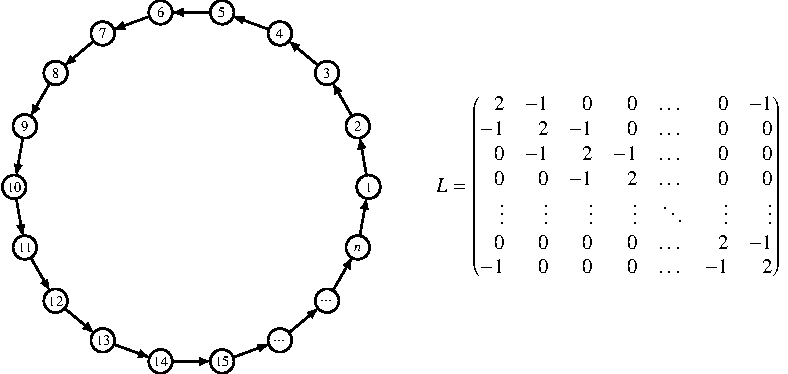
\includegraphics{chapters/70-graphen/images/kreis.pdf}
\caption{Beispielgraph zur Illustration der verschiedenen Basen auf einem
Graphen.
\label{buch:graphen:fig:kreis}}
\end{figure}
Wir illustrieren die im folgenden entwickelte Theorie an dem Beispielgraphen
von Abbildung~\ref{buch:graphen:fig:kreis}.
Für jedes $k=0,\dots,n-1$ ist der Vektor mit den Komponenten
\[
\chi_k(l) = e^{2\pi ikl/n}, \quad l=1,\dots,n
\]
ein Eigenvektor der Laplace-Matrix zum Eigenwert
$\lambda_k=4\sin^2\frac{\pi k}{n}$.
Tatsächlich ist
\begin{align*}
(L\chi_k)(l)
&=
-\chi_k(l-1)
+
2\chi_k(l)
-
\chi_k(l+1)
\\
&=
-e^{2\pi ik(l-1)/n}
+
2e^{2\pi ikl/n}
-
e^{2\pi ik(l+1)/n}
\\
&=
(-e^{-2\pi ik/n}+2-e^{2\pi ik/n})e^{2\pi ikl/n}
\\
&=
-(e^{2\pi ik/2n}-e^{-2\pi ik/2n})^2 \chi_k(l)
\\
&=
-
\biggl(
\frac{e^{2\pi ik/2n}-e^{-2\pi ik/2n}}{2i}
\biggr)^2
(2i)^2 \chi_k(l)
\\
&=
4\sin^2\frac{\pi k}n \chi_k(l)
\end{align*}

Natürlich sind auch Real- und Imaginärteil Eigenvektoren:
\[
\begin{aligned}
s_k(l)
&=
\sin\frac{2\pi kl}{n}
=
\Im \chi_k(l),
\\
c_k(l)
&=
\cos\frac{2\pi kl}{n}
=
\Re\chi_k(l).
\end{aligned}
\]
Das Skalarprodukt dieser Funktionen ist
\[
\langle \chi_m, \chi_{m'}\rangle
=
\frac1n
\sum_{l=1}^n
\overline{e^{2\pi i ml/n}}
e^{2\pi im'l/n}
=
\frac1n
\sum_{l=1}^n
e^{\frac{2\pi i}{n}(m'-m)l}
=
\delta_{mm'}
\]
Die Funktionen bilden daher eine Orthonormalbasis des komplexen
Vektorraums der
komplexen Funktionen auf $G$ mit dem sesquilinearen Skalarprodut.
Wegen $\overline{e_m} = e_{-m}$ folgt, dass für gerade $n$
die Funktionen
\[
c_0, c_1,s_1,c_2,s_2,\dots c_{\frac{n}2-1},c_{\frac{n}2-1},c_{\frac{n}2}
\]
eine orthonormierte Basis des reellen Vektorraumes der reellen Funktionen
auf $G$ mit dem gewöhnlichen Skalarprodukt.

\subsection{Standardbasis und Eigenbasis
\label{buch:subsection:standardbasis-und-eigenbasis}}
Die einfachste Basis, aus der sich Funktionen auf dem Graphen linear
kombinieren lassen, ist die Standardbasis.
Sie hat für jeden Knoten $v$ des Graphen eine Basisfunktion mit den Werten
\[
e_v\colon V\to\mathbb R:v'\mapsto \begin{cases}
1\qquad&v=v'\\
0\qquad&\text{sonst.}
\end{cases}
\]
Sie zeichnet sich dadurch aus, dass sie perfekt lokalisiert ist.
Im Gegensatz dazu zeigt das Beispiel von
Abschnitt~\ref{buch:graphen:subsection:zyklischer-graph}, dass
die Eigenfunktionen von $L(G)$ typischerweise delokalisiert sind.
Im Beispiel hat $\chi_k(l)$ überall auf dem Graphen den gleichen
Betrag.
Die ``Frequenz'' einer Eigenfunktion dagegen ist exakt bestimmt.

\subsection{Fourier-Theorie auf einem Graphen}
Die Eigenfunktionen der Laplace-Matrix auf einem Graphen erlauben
also, das Wärmeleitungsproblem auf dem Graphen auf ganz ähnliche
Art zu lösen, wie die Fourier-Theorie das Wärmeleitungsproblem auf
$\mathbb{R}$ oder auf einem Intervall löst.
Es ist daher angemessen, die Entwicklung einer Funktion
$f\colon G\to\mathbb{C}$ nach den Eigenvektoren $\chi_k$
als Fourier-Transformation zu bezeichnen und die Koeffizienten
\(
c_k = \langle \chi_k, f\rangle
\)
als die Fourier-Koeffizienten.
Grundlegende Eigenschaften der Fourier-Transformation stehen damit
auch für die Analyse von Funktionen auf einem Graphen zur Verfügung.

Es fehlen allerdings Eigenschaften, die mit zusätzlicher Struktur
auf dem Definitionsbereich zusammenhängen.
Die Faltung zum Beispiel setzt eine Rechenoperation auf dem
Definitionsbereich voraus, welche natürlich in einem Graphen nicht erwartet
werden kann.
Im Beispiel von Abschnitt~\ref{buch:graphen:subsection:zyklischer-graph}
lässt sich eine solche Struktur finden, die Knoten des Graphen können
als die Elemente einer zyklischen Gruppe betrachtet werden.
Daraus lassen sich die bekannten Faltungsformeln der diskreten
Fourier-Transformation ableiten.

